\documentclass{standalone}
\usepackage{tikz}
% \usetikzlibrary{shapes.geometric, positioning, arrows.meta}
\usetikzlibrary{arrows.meta, positioning, shapes, decorations.pathreplacing}
\usepackage{palatino} % Use the Palatino font

\begin{document}
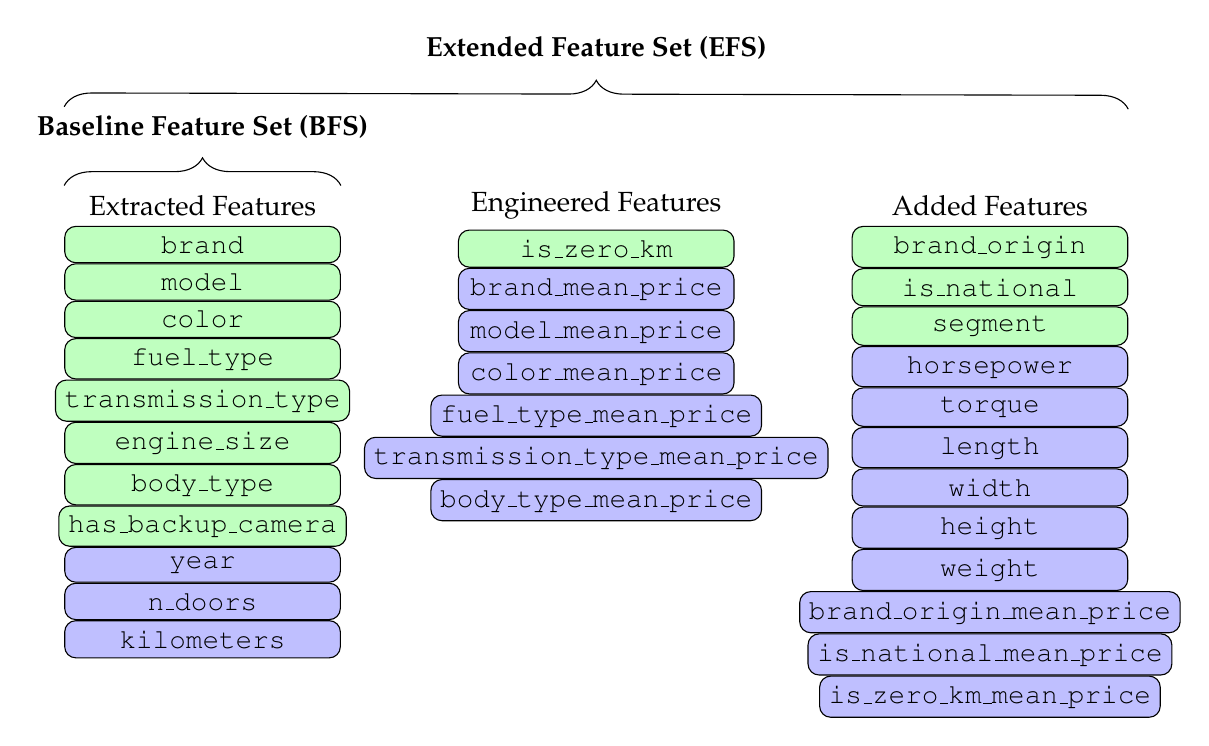
\begin{tikzpicture}[
  node distance=0cm and 2cm,
  every node/.style={draw, rounded corners, align=center},
  categorical/.style={rectangle, minimum width=3.5cm, minimum height=0.25cm, fill=green!25},
  numerical/.style={rectangle, minimum width=3.5cm, minimum height=0.25cm, fill=blue!25},
  brace/.style={decorate, decoration={brace, amplitude=10pt}},
  arrow/.style={->, thick}
]

% Title
\node[draw=none, fill=none] (title1) {\bf{Extended Feature Set (EFS)}};

\node[draw=none, fill=none] (title2) at (-5,-1) {\bf{Baseline Feature Set (BFS)}};

% Features 1
\node[draw=none, fill=none] (features_title_1) at (-5,-2) {Extracted Features};
\node[categorical] (feature1) [below=of features_title_1] {\texttt{brand}};
\node[categorical] (feature2) [below=of feature1] {\texttt{model}};
\node[categorical] (feature3) [below=of feature2] {\texttt{color}};
\node[categorical] (feature4) [below=of feature3] {\texttt{fuel\textunderscore type}};
\node[categorical] (feature5) [below=of feature4] {\texttt{transmission\textunderscore type}};
\node[categorical] (feature6) [below=of feature5] {\texttt{engine\textunderscore size}};
\node[categorical] (feature7) [below=of feature6] {\texttt{body\textunderscore type}};
\node[categorical] (feature8) [below=of feature7] {\texttt{has\textunderscore backup\textunderscore camera}};
\node[numerical] (feature9) [below=of feature8] {\texttt{year}};
\node[numerical] (feature10) [below=of feature9] {\texttt{n\textunderscore doors}};
\node[numerical] (feature11) [below=of feature10] {\texttt{kilometers}};

% Features 2
\node[draw=none, fill=none] (features_title_2) at (0, -2) {Engineered Features};
\node[categorical] (feature12) [below=of features_title_2] {\texttt{is\textunderscore zero\textunderscore km}};
\node[numerical] (feature13) [below=of feature12] {\texttt{brand\textunderscore mean\textunderscore price}};
\node[numerical] (feature14) [below=of feature13] {\texttt{model\textunderscore mean\textunderscore price}};
\node[numerical] (feature15) [below=of feature14] {\texttt{color\textunderscore mean\textunderscore price}};
\node[numerical] (feature16) [below=of feature15] {\texttt{fuel\textunderscore type\textunderscore mean\textunderscore price}};
\node[numerical] (feature17) [below=of feature16] {\texttt{transmission\textunderscore type\textunderscore mean\textunderscore price}};
\node[numerical] (feature18) [below=of feature17] {\texttt{body\textunderscore type\textunderscore mean\textunderscore price}};

% Features 3
\node[draw=none, fill=none] (features_title_3) at (5, -2) {Added Features};
\node[categorical] (feature19) [below=of features_title_3] {\texttt{brand\textunderscore origin}};
\node[categorical] (feature20) [below=of feature19] {\texttt{is\textunderscore national}};
\node[categorical] (feature21) [below=of feature20] {\texttt{segment}};
\node[numerical] (feature22) [below=of feature21] {\texttt{horsepower}};
\node[numerical] (feature23) [below=of feature22] {\texttt{torque}};
\node[numerical] (feature24) [below=of feature23] {\texttt{length}};
\node[numerical] (feature25) [below=of feature24] {\texttt{width}};
\node[numerical] (feature26) [below=of feature25] {\texttt{height}};
\node[numerical] (feature27) [below=of feature26] {\texttt{weight}};
\node[numerical] (feature28) [below=of feature27] {\texttt{brand\textunderscore origin\textunderscore mean\textunderscore price}};
\node[numerical] (feature29) [below=of feature28] {\texttt{is\textunderscore national\textunderscore mean\textunderscore price}};
\node[numerical] (feature30) [below=of feature29] {\texttt{is\textunderscore zero\textunderscore km\textunderscore mean\textunderscore price}};

% Braces
\draw[brace] ([yshift=0.75cm]feature1.west) -- ([yshift=0.75cm]feature1.east);
\draw[brace] ([yshift=1.75cm]feature1.west) -- ([yshift=1.75cm]feature19.east);

\end{tikzpicture}
\end{document}

